%\setchapterpreamble[u]{%
%\dictum[Johann Wolfgang von Goethe]{Es ist nicht genug, zu wissen, man muß auch anwenden; es ist nicht genug, zu wollen, man muß auch tun. \dots}}
\chapter{System- und Softwareentwurf} \index{System- und Softwareentwurf}\label{kap:systemundsoftwarentwurf}


Dieses Kapitel beschreibt den System- und Softwareentwurf sowie die Auswahl der Umgebung, Plattform, Software, Programmiersprache und Frameworks.

\section{Auswahlprozess}
\subsection{Programmiersprache}
Vorgegeben ist die Umsetzung eines Web Services. Da Web Services in fast allen aktuellen Programmiersprachen entwickelt werden können, kann prinzipiell auch jede Sprache ausgewählt werden. 
Es muss die andere technische Voraussetzung erfüllt werden, die vorhandene Oracle PLIB Datenbank abrufen zu können. 

Es wurde die Sprache Java gewählt, da diese zum einen in der aktuellen Industrie stark verbreitet  und zum anderen der Autor dieser Arbeit seit vielen Jahren damit vertraut ist. 

Ein weiterer Aspekt ist, dass Software welche mit Java entwickelt wurde im Prinzip auf jeder Plattform lauffähig ist. 

\section{Softwaredesign und Architektur}

Dieses Kapitel gibt einen Überblick über das Softwaredesign und die Architektur des Systems. 

\subsection{Bausteinsicht}
\begin{quotation}
Die Bausteinsicht bildet die Aufgaben des Systems auf Software-Bausteine oder -Komponenten ab.
 \citep[S. 98ff][]{starke}	
\end{quotation}

Es soll mit Hilfe dieser Sicht ein Überblick über den Aufbau des Systems und den Abhängigkeiten der einzelnen Komponenten geschaffen werden. Dazu wird das System im top-down Ansatz aufgezeigt und verfeinert. 

\subsubsection{Level 0 - Systemüberblick mit angrenzenden Systemen} 



\begin{figure}[htbp]
	\centering
		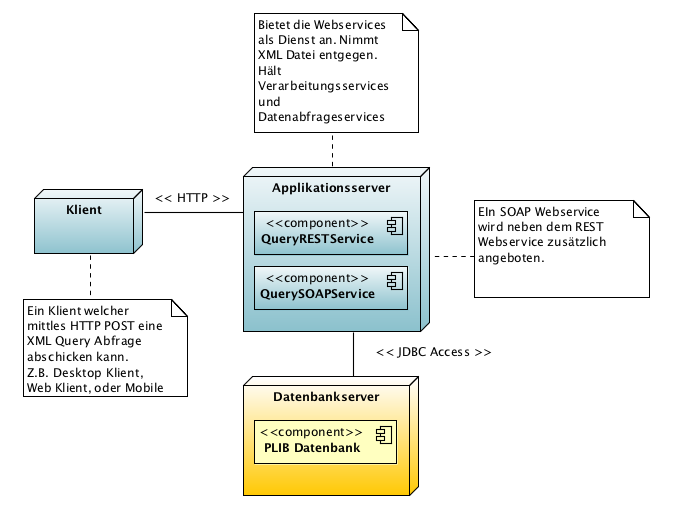
\includegraphics[width=0.9\textwidth]{images/bausteinsicht_plib_level0.png}
	\caption{Bausteinsicht Level 0}
	\label{fig:bausteinsicht_level0}
\end{figure}

\paragraph{Klient}

Der Klient stellt den Nutzer des Query Services dar. Er erzeugt das XML File, welches als Query an den Service geschickt wird. Der Transport erfolgt über das HTTP Protokoll.  

\paragraph{Applikationsserver}

Der Applikationsserver ist der Hauptbaustein. Dieser Baustein enthält alle entwickelten Komponenten. Sichtbar von außen ist der QueryService, dieser Service ist ein REST WebService und nimmt XML-Dateien als POST Request entgegen. 

\subsubsection{Level 1 - Plib characteristic query} 

Die Bausteinsicht Level 1 zeigt alle Komponenten des entwickelten Systems auf und deutet die externen Schnittstellen an. Mittels <<use>> Beziehungen erkennt man die Abhängigkeiten der einzelnen Komponenten. 

\begin{figure}[htbp]
	\centering
		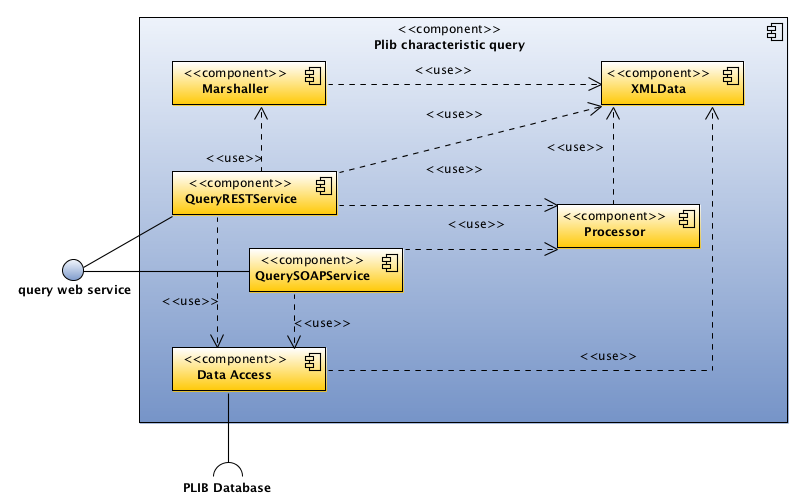
\includegraphics[width=0.98\textwidth]{images/bausteinsicht_plib_level1.png}
	\caption{Bausteinsicht - Level 1}
	\label{fig:bausteinsicht_level1}
\end{figure}

\begin{description}
\item[QueryService] Der Zweck dieser Komponente ist das entgegennehmen des Requests (Query-XML File), das Weiterleiten an die entsprechenden Weiterverarbeitenden Komponenten und letztlich das Zurücksenden der Rückantwort (Katalog-XML).
\item[Data Access] Diese technische Komponente beinhaltet die Zugriffsschicht auf die externe Datenbankschnittstelle und bietet entsprechend vereinfachte Abfrageschnittstellen für die anderen Komponenten an. 
\item[Marshaller] Eine weitere technische Komponente, diese ist für das Einlesen und Validieren der eingegangenen Query-XML Datei verantwortlich. Ferner transformiert diese Komponente die Informationen aus der Query-XML nach Validierung in das im System benutze Datenmodell aus der Komponente XMLData.
\item[XMLData] Beinhaltet das Datenmodell des Systems. Sowohl die eingehenden Query-XML Daten, als auch die ausgehenden Katalog-XML Daten werden intern in ein entsprechendes Model zur Verarbeitung abgelegt, so dass darauf gearbeitet werden kann.  
\item[Analyser] XXX
\item[Handler] XXX
\end{description}

\subsubsection{Level 2 - Whiteboxansicht - Komponente XMLData} 

Die Komponente XMLData beinhaltet alle Datenmodelle für die beiden Hauptkonzepte "Query for characteristic data" nach 

\begin{figure}[htbp]
	\centering
		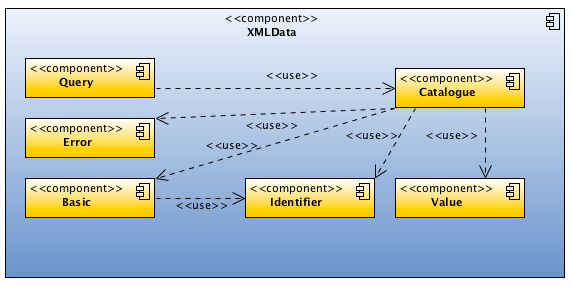
\includegraphics[width=0.82\textwidth]{images/bausteinsicht_plib_level2_xmldata.png}
	\caption{Bausteinsicht - Level 2 - Komponente XMLData}
	\label{fig:bausteinsicht_level2_xmldata}
\end{figure}

\begin{description}
\item[Query] Diese Komponente beinhaltet das Datenmodell des Queries nach ISO/TS 29002-31. 
\item[Catalogue] Diese Komponente beinhaltet das Datenmodell des Kataloges nach ISO/TS 29002-10. 
\item[Basic] Diese Komponente beinhaltet das Datenmodell von Basistypen nach ISO/TS 29002-4.
\item[Value] Diese Komponente beinhaltet das Datenmodell der Wertetypen nach ISO/TS 29002-10.
\item[Identifier] Diese Komponente beinhaltet das Datenmodell für Identifier (IRDI) nach ISO/TS 29002-5. 
\end{description}

\subsection{Klassendiagramm}

\begin{figure}[htbp]
	\centering
		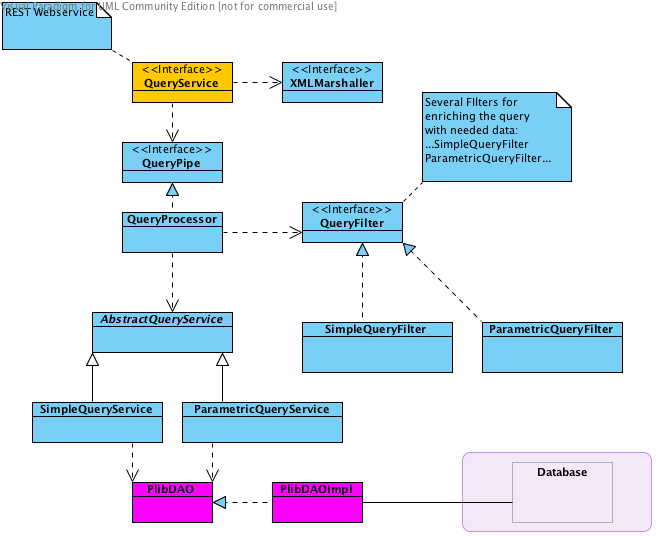
\includegraphics[width=0.98\textwidth]{images/klassendiagramm_plib.png}
	\caption{Klassendiagramm}
	\label{fig:klassendiagramm}
\end{figure}
